\subsection{Teilaufgabe 2}
\subsubsection{Aufgabenstellung}
In dieser Teilaufgabe sollen wir ein Programm schreiben welle die Wertebereiche der primitieven
Datentypen ausgibt.

\subsubsection{Anforderungsdefinition}
\begin{enumerate}
	\item Zu jedem primitieven Datentypen den Max und Min-Wert ausgeben.
\end{enumerate}

\subsubsection{Entwurf}
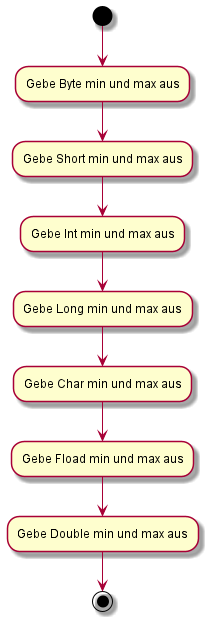
\includegraphics[scale=0.75]{uml/uml_c3_p1.png}

\subsubsection{Quelltext}
\paragraph{Wertebereiche.java}\
\lstinputlisting[language = Java , frame = trBL , escapeinside={(*@}{@*)}]{../chapter_03/src/chapter_03/Wertebereiche.java}


\subsubsection{Testdokumentation}
Nach dem start des Programmes sollten die Min und Max werte der einzelnen Datentypen ausgegeben
werden, dies ware auch der Fall.

\subsubsection{Benutzungshinweise}
Keine Besonderen Benutzungshinweise.
Man navigiere zu dem Ordner von sich die Compilierte Datei mit dem Namen "Wertebereiche.class"
\space befindet und führt anschlie\ss end java Wertebereiche aus.

\subsubsection{Anwendungsbeispiel}
Nach dem man das Programm gestartet hat, sollte folgende Ausgabe erscheinen:
\begin{lstlisting}[frame = trBL , firstnumber = last , escapeinside={(*@}{@*)}]
[sebastian@laptop bin]$ java Wertebereiche
Byte min -128 | Byte max 127
Short min -32768 | Short max 32767
Integer min -2147483648 | Integer max 2147483647
Long min -9223372036854775808 | Byte Long 9223372036854775807
Char min  | Char max ￿
Float min 1.4E-45 | Float max 3.4028235E38
Double min 4.9E-324 | Double max 1.7976931348623157E308
[sebastian@laptop bin]$ 
\end{lstlisting}